\documentclass[border=10pt]{standalone}

\usepackage{tikz}
\usepackage{tikzsymbols}
\usetikzlibrary{calc,patterns,shapes.geometric}

\def\centerarc[#1](#2)(#3:#4:#5){\draw[#1] ($(#2)+({#5*cos(#3)},{#5*sin(#3)})$) arc (#3:#4:#5);}

\begin{document}
	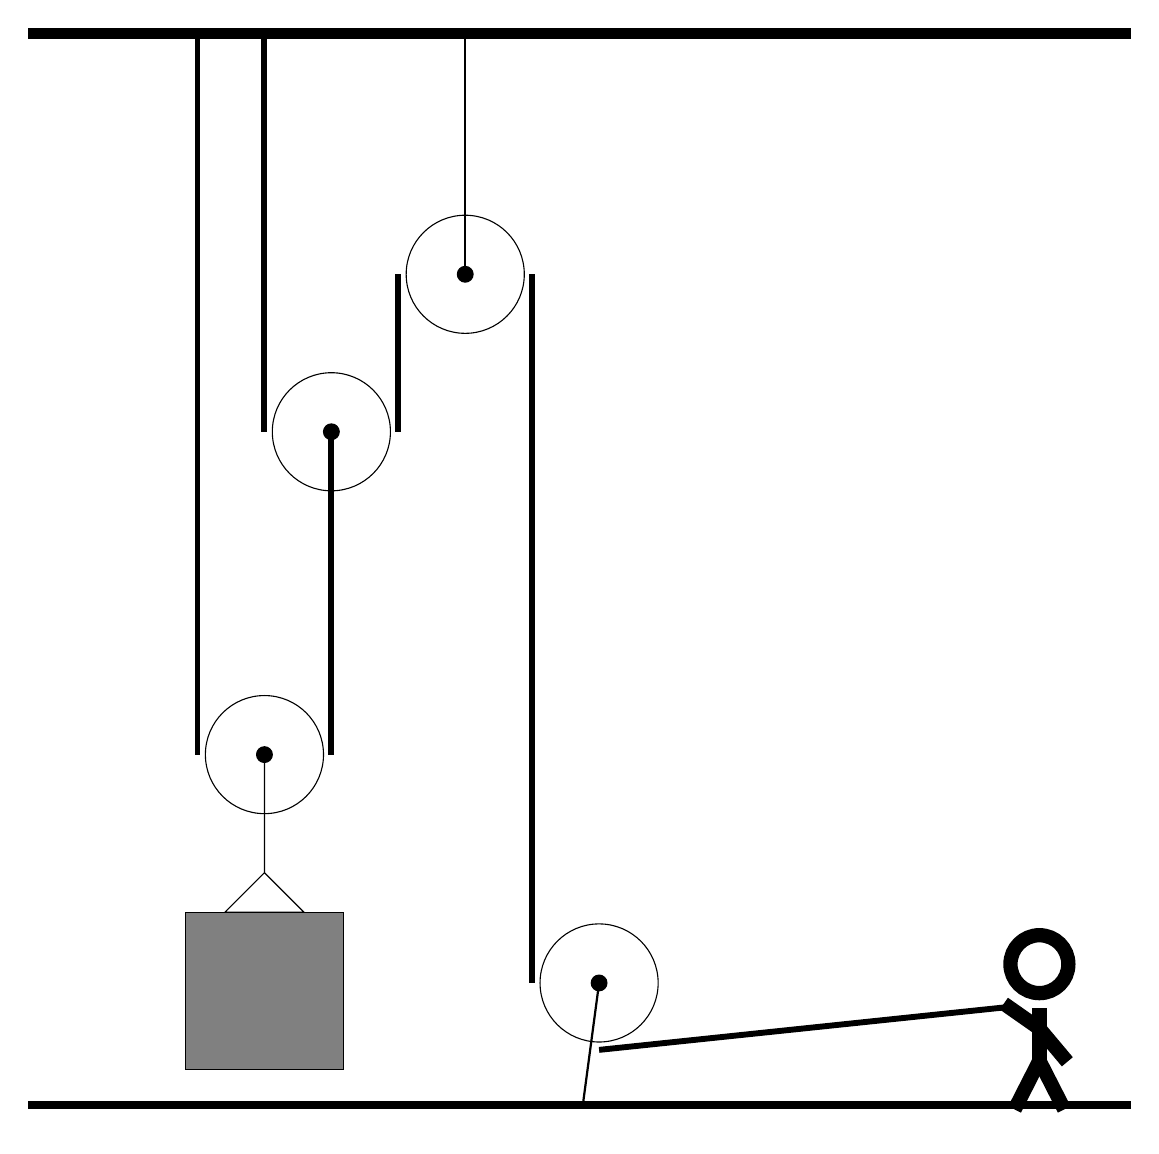
\begin{tikzpicture}
		%%%%% START %%%%%
		\draw[fill=black] (-2, 10) rectangle (12, 10.125);
		
		\draw (1, 0.9) circle (0.75);
		\draw[fill=black] (1, 0.9) circle (0.1);
		
		\draw (1.85, 5.0) circle (0.75);
		\draw[fill=black] (1.85, 5.0) circle (0.1);
		
		\draw (3.55, 7.0) circle (0.75);
		\draw[fill=black] (3.55, 7.0) circle (0.1);
		\draw[thick] (3.55, 7.0) -- (3.55, 10);
		
		\draw (5.25, -2) circle (0.75);
		\draw[fill=black] (5.25, -2) circle (0.1);
		\draw[thick] (5.25, -2) -- (5.05, -3.5);
		
		\draw (1, 0.9) -- (1, -0.6) -- (0.5, -1.1) -- (1.5, -1.1) -- (1, -0.6);
		\draw[fill=black!50] (0, -1.1) rectangle (2, -3.1);
		\draw[line width=0.75mm] (0.15, 10) -- (0.15, 0.9);
		\centerarc[line width=0.75mm](1, 0.9)(180:360:0.85);
		\draw[line width=0.75mm](1.85, 0.9) -- (1.85, 5.0);
		\draw[line width=0.75mm] (1.0, 10) -- (1.0, 5.0);
		\centerarc[line width=0.75mm](1.85, 5.0)(180:360:0.85);
		\draw[line width=0.75mm](2.7, 5.0) -- (2.7, 7.0);
		\centerarc[line width=0.75mm](3.55, 7.0)(0:180:0.85);
		\draw[line width=0.75mm] (4.4, 7.0) -- (4.4, -2);
		\centerarc[line width=0.75mm](5.25, -2)(0:90:-0.85);
		\draw[line width=0.75mm](5.25, -2.85) -- (10.5, -2.3);
		
		\node at (10.8, -2.5) {\Strichmaxerl[10][-35][-50]};
		
		\draw[fill=black] (-2, -3.5) rectangle (12, -3.6);
		%%%%% END %%%%%
	\end{tikzpicture}
\end{document}